\documentclass[12pt,a4paper]{article}
\usepackage[utf8]{inputenc}
\usepackage[francais]{babel}
\usepackage[T1]{fontenc}
\usepackage{graphicx}


\usepackage{lipsum}
\usepackage{listings}
\usepackage{enumerate}
\usepackage[backend=bibtex8,backref=true]{biblatex}

\newcommand{\MONTITRE}{La virtualisation avec Proxmox}
\newcommand{\MONSOUSTITRE}{Installation et confuguration}

\addbibresource{dimitri_guedin.bib}
\defbibcheck{online}{\iffieldundef{url}{\skipentry}{}}
\defbibcheck{notonline}{\iffieldundef{url}{}{\skipentry}}

\title{
\begin{tabular}{p{3.5cm} r}
& {\Huge {\bf \MONTITRE}}\\
& {\huge \MONSOUSTITRE}\\
& version du \today{}
\end{tabular}
}


\begin{document}
\maketitle
\newpage
\tableofcontents{}
\newpage

\section{Architecture de la solution}
Le projet consiste à crée un site web qui nous servira de portefeuille de compétences dans le cadre du BTS SIO (Services Informatiques aux Organisations). \\

Le site étant héberger à domicile nous devons donc crée notre propre serveur et en faire la configuration. Nous avons donc choisi de nous tourner vers des solutions libre pour mené a bien ce projet.\\



Ce projet englobe donc les deux spécialités de notre BTS, à savoir développement et réseau. La sécurité des serveurs sera une partie importante car nous allons ouvrir le site sur l'extérieur, pour cela nous utiliserons plusieurs outils notamment Nagios pour la supervision des serveurs, failtoban pour la prévention des intrusions et nous sécuriseront nos serveur avec des certificats SSL.\\

\textbf{La virtualisation}\newline
Pour des raisons économiques nous avons virtualisée le serveur web, la plateforme de virtualisation que nous avons choisi est nommée Proxmox qui est un système basé sur une distribution Debian.\\

\textbf{Le serveur web}\newline
Le système d'exploitation qui nous servira de serveur web sera un système GNU/Linux, la distribution Debian. Sur ce serveur nous ajouterons un serveur FTP qui sera par la suite sécurisé.\\

\textbf{Le serveur de base de données}\newline
Nous avons décidé pour des raisons de sécurité de ne pas inclure la base de données du site dans le serveur web, nous allons donc mettre un place un deuxième serveurs ou nous utiliserons une Raspberry Pi pour l'hébergement du serveur de base de données.\\

\newpage
\section{Proxmox: Serveur de machines virtuelles}

Proxmox VE est une solution open source complète de virtualisation pour serveurs. Il est basé sur les technologies de virtualisation KVM et conteneurs et gère les machines virtuelles, le stockage, les réseaux virtualisés, et la haute disponibilité.

Les fonctionnalités avancées et l'interface Web intuitive sont conçues pour vous aider à optimiser l'utilisation de vos ressources existantes, réduire les coûts en matériel et le temps nécessaire à l'administration - en entreprise ainsi qu'à la maison. Vous pouvez facilement virtualiser les charges de travail les plus élevées sous Linux et Windows.
\newpage
\section{Installation}

\begin{figure}[!ht]
\center
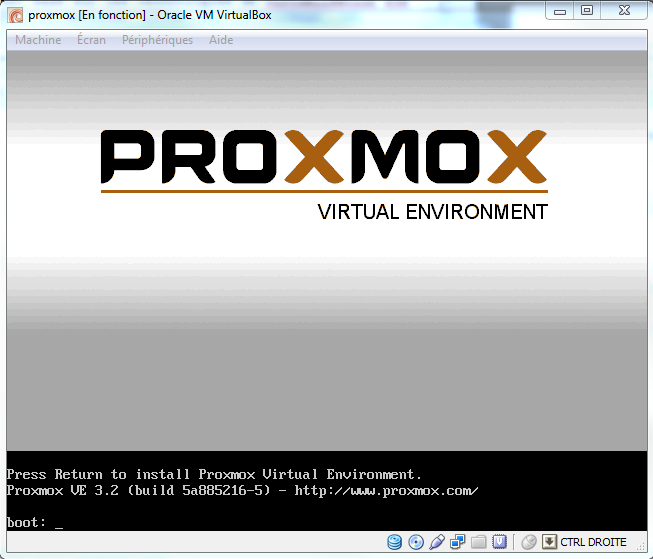
\includegraphics[width=9cm]{Images/1.PNG} 
\caption{Ecran de boot}
\end{figure}

\begin{center}
Pour commencer l'installation de Proxmox il faut appuyer sur la touche "entrée"
\end{center}

\begin{figure}[!ht]
\center
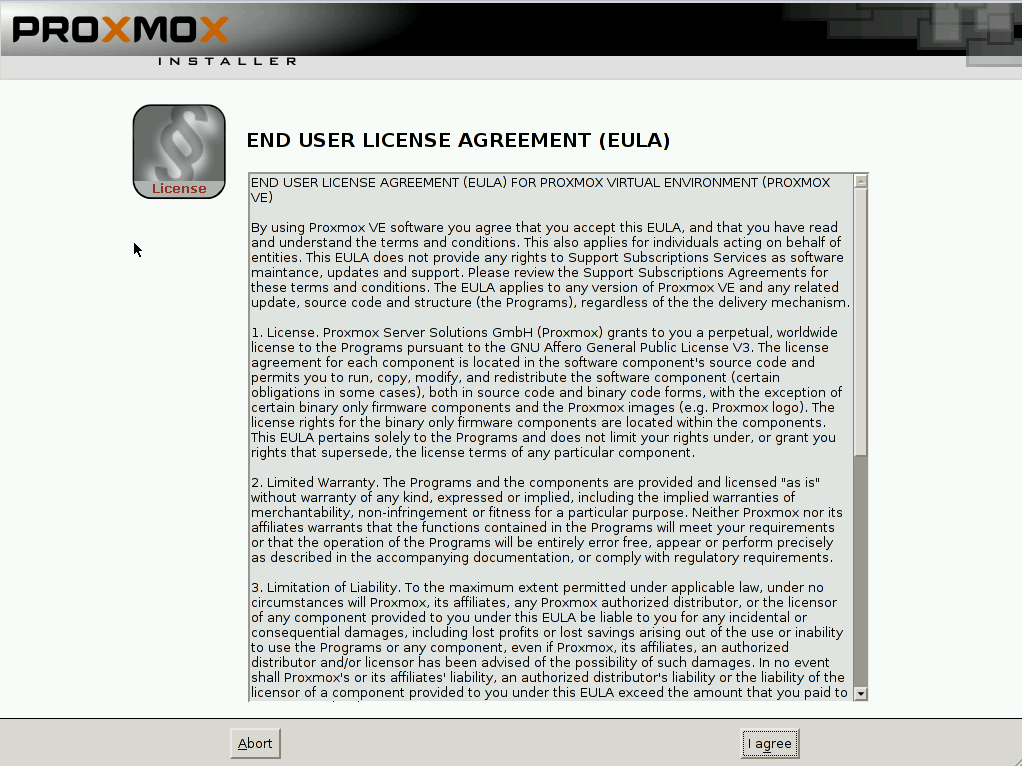
\includegraphics[width=9cm]{Images/2.PNG} 
\caption{Accepter les conditions en cliquant sur "I agree"}
\end{figure}

\begin{figure}[!ht]
\center
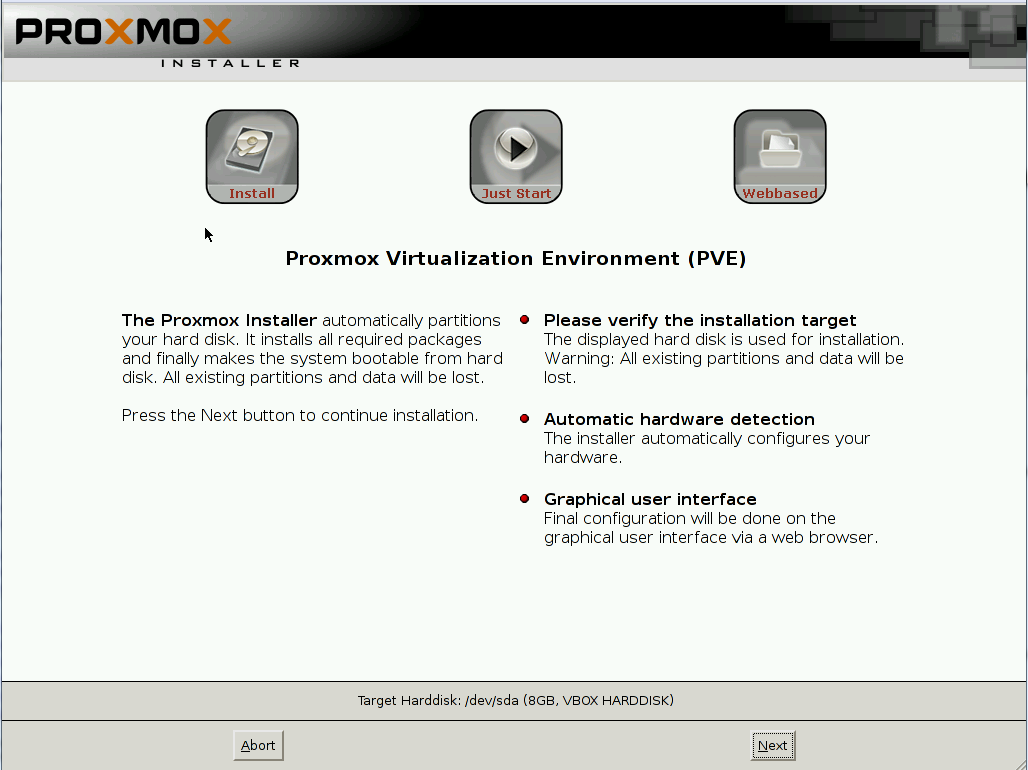
\includegraphics[width=10cm]{Images/3.PNG}  
\caption{Choix du disque}
\end{figure}

\begin{center}
Je rappel que nous somme sur un environnement VirtualBox je n'ai alors qu'un choix de disque dur, sur une machine physique composée de plusieurs disque dur il y aura donc plusieurs choix de disque. 
\end{center}

\begin{figure}[!ht]
\center
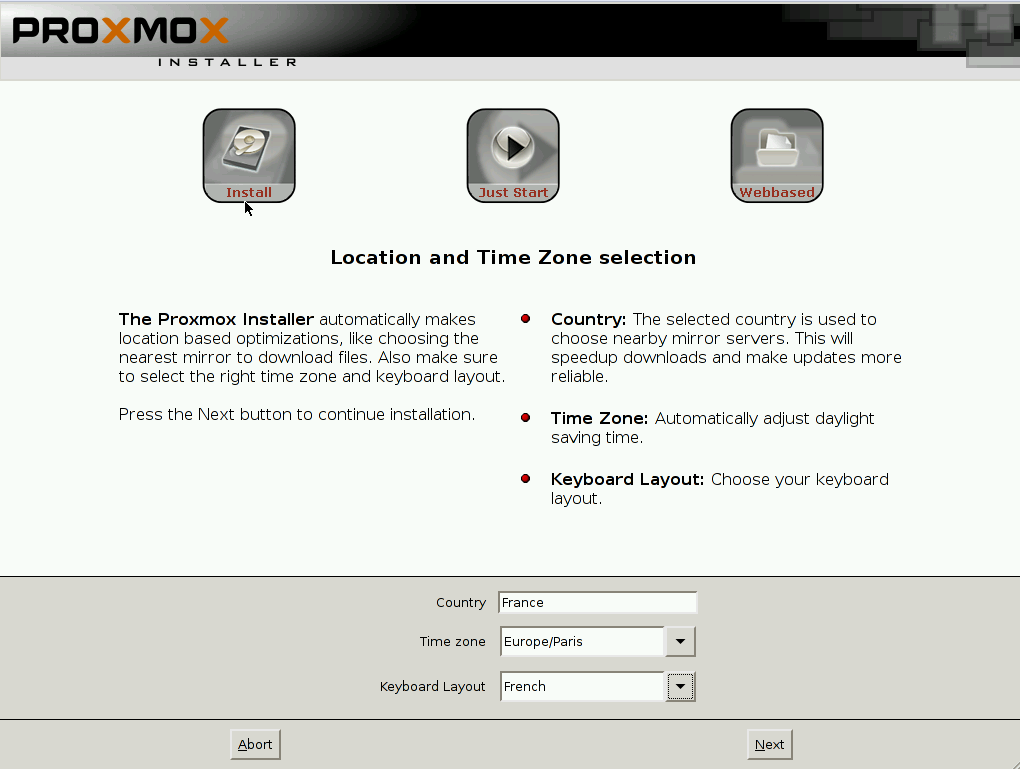
\includegraphics[width=9cm]{Images/4.PNG}  
\caption{Localisation et choix du clavier}
\end{figure}

\begin{center}
Dans cette partie vous aurai a choisir votre pays ainsi que le mode de clavier que vous désiré.\\
\end{center}

\begin{figure}[!ht]
\center
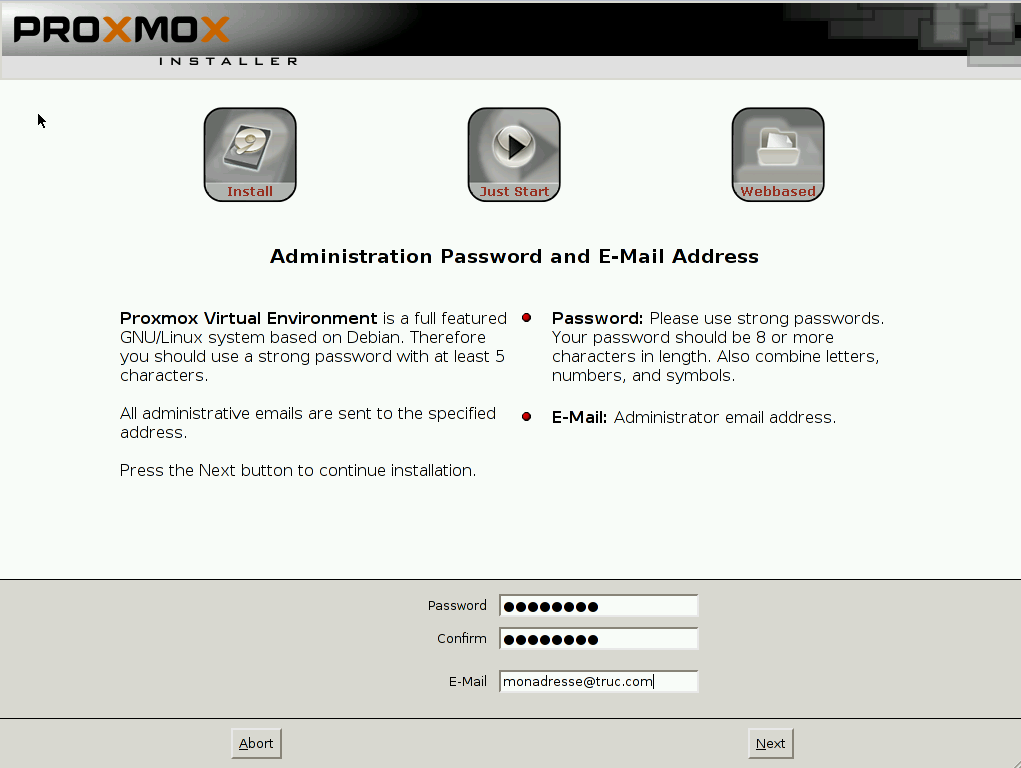
\includegraphics[width=9cm]{Images/5.PNG}  
\caption{Mot de passe et adresse mail ADMIN}
\end{figure}

\begin{center}
Pour cette partie le mot de passe sera le mot de passe pour l'utilisateur "root" c'est a dire l'administrateur disposant des plein droit sur le serveur Proxmox. 
\end{center}

\begin{figure}[!ht]
\center
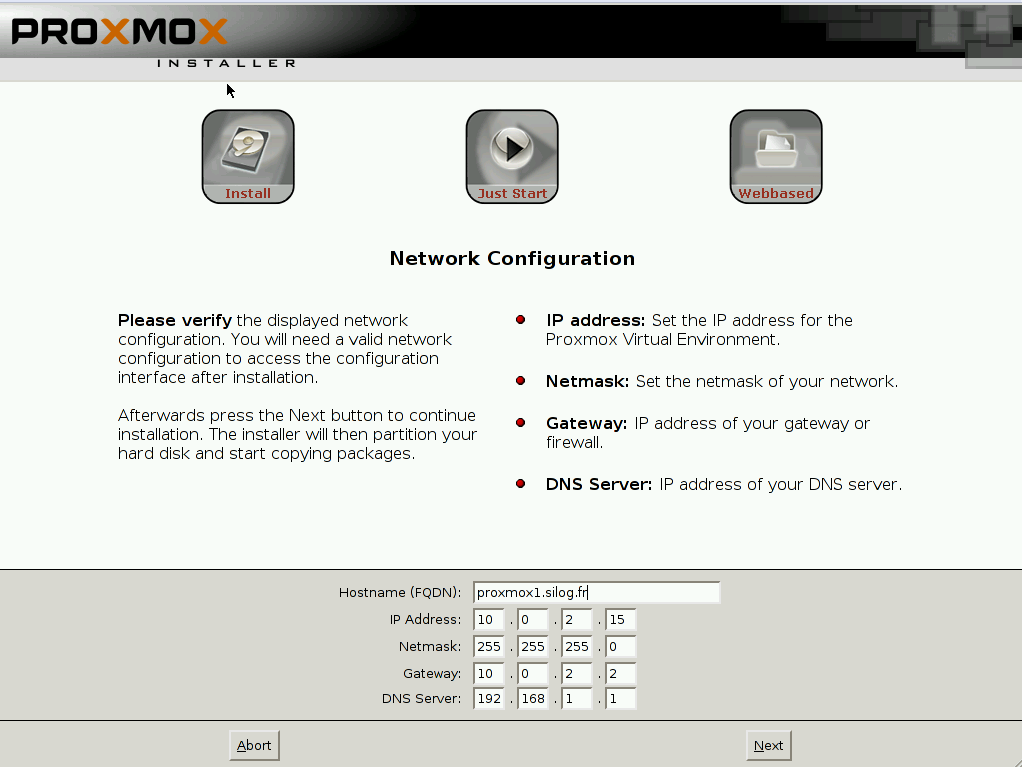
\includegraphics[width=8cm]{Images/6.PNG}  
\caption{Configuration réseau}
\end{figure}

\begin{center}
Pour finir les configurations réseau de proxmox avec l'adresse IP de votre machine. Pour ce qui est du miroir vous j'ai pris celle ci: 
\textit{proxmox1.silog.fr} Il ne vous reste plus qu'a entrer l'adresse IP de votre serveur dans un navigateur 
\textbf{\textit{ex: https://192.168.X.X:8006}}
\end{center}

\newpage
\section{Création de compte utilisateur}

Par défaut sur Proxmox nous avons un seul utilisateur, root, qui dispose des pleins droit sur tout le système. Nous allons donc voir dans cette partie comment crée de nouveau utilisateur soit en ligne de commande ou alors avec Webmin de façon graphique.

\subsection{En ligne de commandes avec Putty}
\textbf{PuTTY} est un émulateur de terminal doublé d'un client pour les protocoles SSH, Telnet, rlogin, et TCP brut. Il permet également d'établir des connexions directes par liaison série RS-232. À l'origine disponible uniquement pour Windows, il est à présent porté sur diverses plates-formes Unix 

\begin{figure}[!ht]
\center
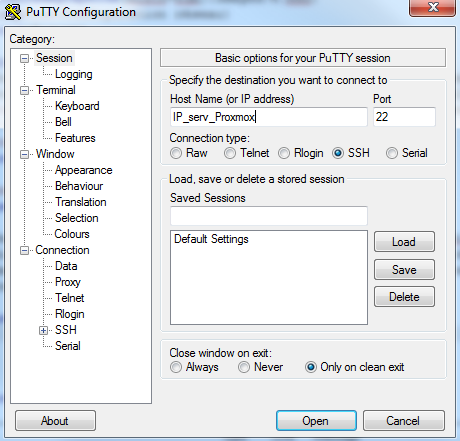
\includegraphics[width=10cm]{Images/7.PNG}  
\caption{Putty}
\end{figure}

\newpage
Pour la connexion à notre serveur Proxmox nous allons utiliser le protocole SSH (Secure Shell) qui permet une connexion sécurisé sur notre serveur.

Une fois l'adresse IP du serveur proxmox entrée un terminal apparaît, nous allons donc nous connecter en root pour crée les nouveaux utilisateurs.

\begin{figure}[!ht]
\center
\includegraphics[width=10cm]{Images/8.PNG}  
\caption{Connexion en SSH sur le serveur}
\end{figure}




\end{document}
